Die Parameter werden nach dem physikalischen Ersatzschaltbild des
Bipolartransistors ohne parasitäre Kapazitäten bestimmt. Bei der
Kleinsignalanalyse werden alle Kapazitäten sowie Spannungsquellen als
Kurzschlüsse behandelt.

\subsubsection{Emitterschaltung}

\begin{figure}[H]
  \begin{center}
    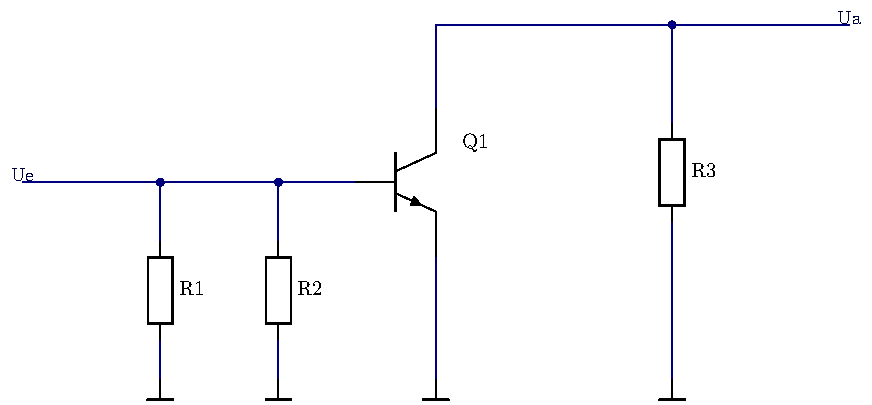
\includegraphics[width=0.618\textwidth]{circuits/commonEmitter_ESB1.pdf}
  \end{center}
  \caption{Kleinsignalersatzschaltbild der Emitterschaltung (Abb. 3)}
\end{figure}

\begin{figure}[H]
  \begin{center}
    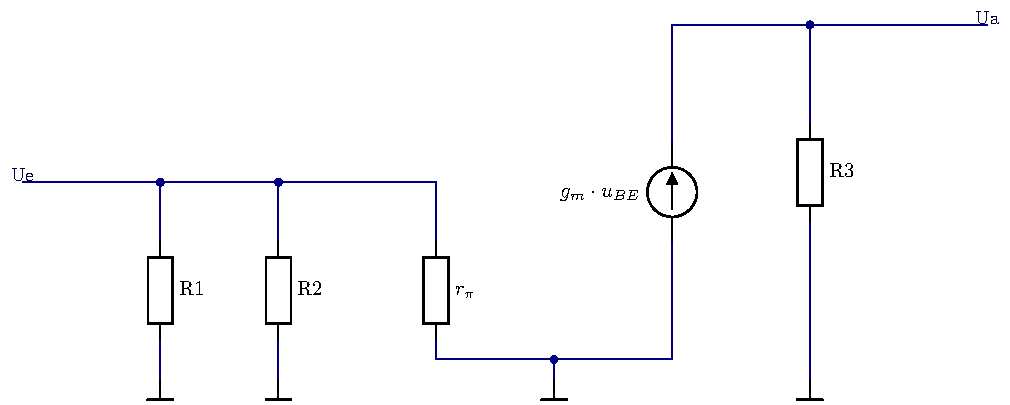
\includegraphics[width=0.618\textwidth]{circuits/commonEmitter_ESB2.pdf}
  \end{center}
  \caption{ESB Abb. 6, Transistor durch phys. ESB ersetzt}
\end{figure}

\noindent Eingangswiderstand:
\[r_e = \frac{U_e}{I_e} = R_1 // R_2 // r_\pi\]
\noindent Ausgangswiderstand:
\[r_a = \frac{U_a}{I_a} = r_0 // R_3 \]
\noindent Spannungsverstärkung:
\[V_u = \frac{U_2}{U_1}\]

\begin{gather*}
  U_2 = g_m \cdot u_{BE} \cdot (r_0 // R_3) = g_m \cdot U_1 \cdot (r_0 // R_3)\\
  V_u = g_m \cdot (r_0 // R_3)
\end{gather*}

\noindent Stromverstärkung:
\[V_i = \frac{I_2}{I_1}\]
\[I_1 = \frac{U_1}{r_\pi} + U_1 (\frac{1}{R_2} + \frac{1}{R_1})\]
\[I_B = \frac{U_1}{r_\pi} = I_1 - U_1 (\frac{1}{R_2} + \frac{1}{R_1})\]
\[I_2 = g_m \cdot U_1 \rightarrow U_1 = \frac{I_2}{g_m}\]
\[ \frac{I_2}{g_m \cdot r_\pi}  = I_1 - \frac{I_2}{g_m} (\frac{1}{R_2} + \frac{1}{R_1}) \]
\[ \frac{1}{g_m \cdot r_\pi}  = \frac{I_1}{I_2} - \frac{1}{g_m} (\frac{1}{R_2} + \frac{1}{R_1}) \]
\[\frac{I_2}{I_1} = V_i = \frac{1}{ \frac{1}{g_m} (\frac{1}{r_\pi} +
    \frac{1}{R_2} + \frac{1}{R_1}) }\]

\noindent Leistungsverstärkung:
\[V_p = \frac{P_2}{P_1} = \frac{U_2 \cdot I_2}{U_1 \cdot I_1} = V_u \cdot V_i\]
\[V_p = \frac{g_m^2 \cdot (r_0 // R_3)}{\frac{1}{r_{\pi}} + \frac{1}{R_2} + \frac{1}{R_1}}\]

%%%%%%%%%%%%%%%%%%%%%%%%%%%%%%%%%%%%%%%%%
\subsubsection{Kollektorschaltung}
\begin{figure}[H]
  \begin{center}
    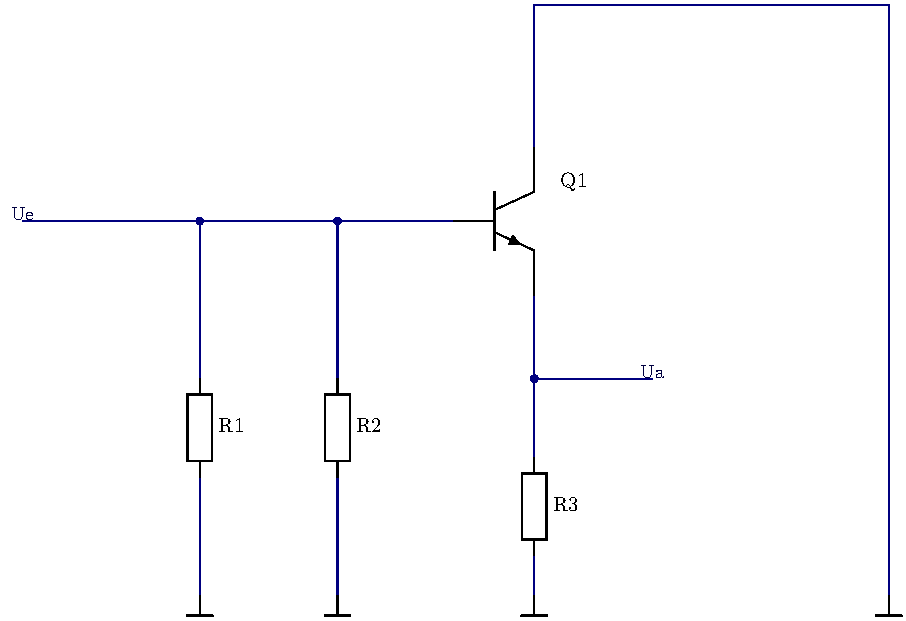
\includegraphics[width=0.618\textwidth]{circuits/commonCollector_ESB1.pdf}
  \end{center}
  \caption{Kleinsignalersatzschaltbild der Kollektorschaltung (Abb. 4)}
\end{figure}


\begin{figure}[H]
  \begin{center}
   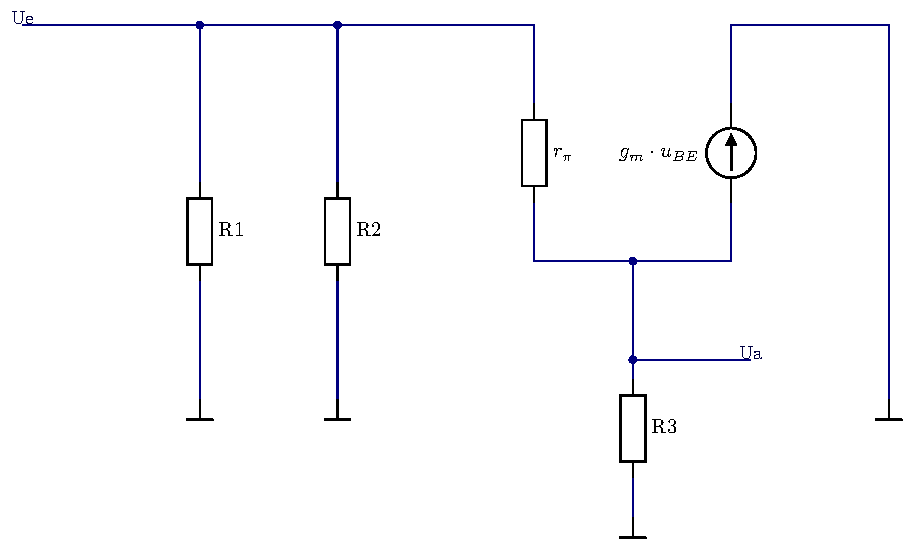
\includegraphics[width=0.618\textwidth]{circuits/commonCollector_ESB2.pdf}
  \end{center}
  \caption{ESB Abb. 8, Transistor durch phys. ESB ersetzt}
\end{figure}
\noindent Eingangswiderstand
\[ r_e = \frac{U_1}{I_1}\]
\[ r_e = R_1 // R_2 // (r_\pi + \beta_N R_3)\]

\noindent Ausgangswiderstand
\[ r_a = \frac{U_2}{I_2}|_{U_1 = 0}\]
\[U_2 = U_{BE}\]
\[r_a = R_3 // \frac{r_\pi }{\beta_N + 1}\]
\[r_a \approx \frac{1}{g_m}\]

\noindent Spannungsverstärkung
\[ V_u = \frac{U_2}{U_1}\]
\[V_u = \frac{1}{1+ \dfrac{1}{g_m \cdot R_3}} \approx 1\]

%%%%%%%%%%%%%%%%%%%%%%%%%%%%%%%%%%%%%%%%%
\subsubsection{Basisschaltung}
\begin{figure}[H]
  \begin{center}
    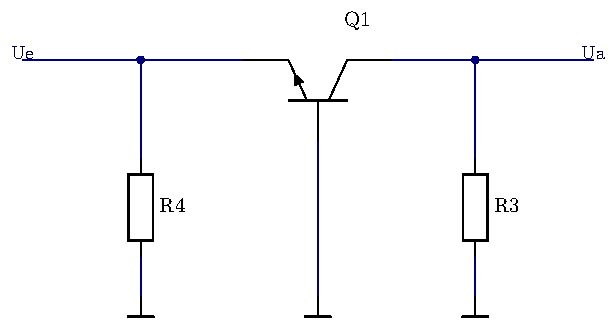
\includegraphics[width=0.618\textwidth]{circuits/commonBase_ESB1.pdf}
  \end{center}
  \caption{Kleinsignalersatzschaltbild der Basisschaltung (Abb. 5)}
\end{figure}

\begin{figure}[H]
  \begin{center}
    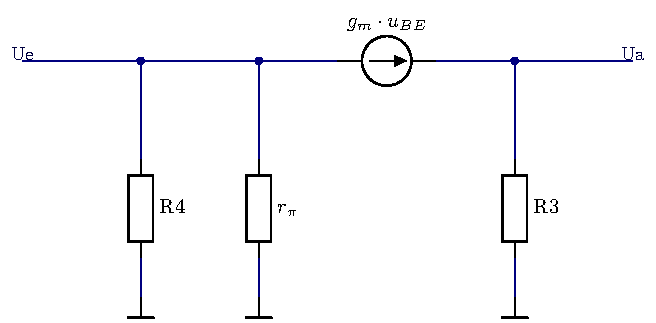
\includegraphics[width=0.618\textwidth]{circuits/commonBase_ESB2.pdf}
  \end{center}
  \caption{ESB Abb. 10, Transistor durch phys. ESB ersetzt}
\end{figure}

\noindent Eingangswiderstand
\[ r_e = \frac{U_1}{I_1}\]
\[0 = I_1 + \frac{U_1}{R_4} + \frac{U_1}{r_\pi} + g_m U_{BE} \]
\[I_1 = - \frac{U_1}{R_4} - \frac{U_{BE}}{r_\pi} - g_m U_{BE} \]
\[U_{BE} = - U_1\]
\[I_1 = \frac{U_1}{R_4} + \frac{U_1}{r_\pi} + g_m U_{1} \]
\[ \frac{I_1}{U_1} = \frac{1}{R_4} + \frac{1}{r_\pi} + g_m \]
\[ r_e = \frac{1}{ \frac{1}{R_4} + \frac{1}{r_\pi} + g_m} \]
\[g_m = \frac{B_n}{r_\pi}\]
\[ r_e = \frac{1}{\frac{1}{R_4} + \frac{1}{r_\pi} (1+B_N)} \]
\[ r_e = \frac{1}{R_4} // (r_\pi (\frac{1}{1+B_N}))\]

\noindent Ausgangswiderstand
\[ r_a = \frac{U_2}{I_2}|_{U_e = 0}\]
\[ I_2 = g_m U_{BE} + \frac{U_2}{R_3 // r_0}\]
\[ U_{BE} = 0\]
\[ r_a = R_3 // r_0\]

\noindent Spannungsverstärkung
\[V_u = \frac{U_2}{U_1}\]
\[U_2 = -g_m \cdot U_{BE} (R_3 // r_0)\]
\[U_{BE} = - U_{1}\]
\[ \frac{U_2}{U_1} = V_u = g_m (R_3 // r_0)\]